\chapter{L'azienda}
\label{cap:lazienda}


\section\azienda

\subsection{Descrizione}
L'azienda {\azienda}, fondata nel 1984, offre servizi di consulenza e sviluppo di software. 
Si è distinta nell'ideazione, costruzione e implementazione di strumenti software per oltre 2500 imprese, 
molte delle quali all'estero. \\
Una delle sue qualità distintive è l'attenzione verso i clienti, 
con vari uffici in regioni come Veneto, Lombardia, Emilia-Romagna, Friuli-Venezia Giulia, Toscana, Puglia e Campania, 
impiegando oltre 600 professionisti. \\
La sede centrale per la ricerca e sviluppo (CSV) si trova a Grisignano di Zocco (VI) e ospita più di 200 collaboratori. 
Qui, gruppi di sviluppatori 
e tecnici lavorano insieme per assicurare servizi affidabili e soluzioni software su misura. 
\newpage

\subsection{Organizzazione dell'azienza e i suoi prodotti}
{\azienda} è suddivisa in \textit{Business Unit} (BU), una parte di un'azienda che opera in modo autonomo o semi-autonomo, 
con la propria visione, \textit{mission}, obiettivi e strategie. Essa ha una propria \textit{leadership} e una struttura 
organizzativa separata, ed è responsabile del proprio profitto e perdite. \\
Le BU possono focalizzarsi su 
specifici mercati geografici, gruppi di clienti o linee di prodotti, permettendo all'azienda di essere 
più agile e rispondere meglio alle esigenze del mercato e dei clienti.\\
In {\azienda} BU sono 11 e, come rappresentate in figura \ref{fig:organizzazione-azienda}, si suddividono in:
\begin{itemize}
  \item \textbf{JGALILEO:} ha sviluppato l’\gls{ERP} –  Jgalileo, il sistema gestionale completo che consente alle imprese di monitorare e governare i flussi aziendali in modo semplice ed efficace, grazie a workflow condivisi e informazioni univoche e coerenti. Il software gestionale ERP Jgalileo si rivolge a tutte le aziende produttive e commerciali di ogni dimensione, dalla piccola azienda al grande gruppo aziendale internazionale, grazie anche alla gestione accurata delle fiscalità estere;
  \item \textbf{NEXTBI:} specializzata in \textit{Information Technology} e consulenza direzionale, con un focus nelle aree \textit{marketing}, vendite, \textit{retail}, \textit{customer innovation}, Business Intelligence, Corporate Performance Management e per le soluzioni \gls{IoT};
  \item \textbf{4WORDS:} specializzata in soluzioni \gls{B2B}, app e \gls{CRM}, ha l’obiettivo di far crescere le aziende grazie a soluzioni digitali dedicate: portale B2B, \gls{app} custom, app per la rete vendita e l’assistenza tecnica, ma anche realtà aumentata e \gls{PIM};
  \item \textbf{TCE:} si occupa di ottimizzare la fase di preventivazione e di acquisizione dell’ordine; \\
  Sviluppa il prodotto \gls{CPQg}, strumento essenziale ai fini della configurazione dell’offerta, 
  della gestione della trattativa e del recepimento del contratto, completo di tutti i contenuti documentali necessari.
  Attraverso uno strumento CPQ la forza vendite può configurare l’offerta più idonea in autonomia, in funzione delle specifiche esigenze del momento, senza preoccuparsi delle complesse logiche commerciali che la piattaforma gestisce in automatico;
  \item \textbf{DISCOVERY QUALITY:} produce una soluzione di Governance aziendale per gestire in modo efficace tutti i processi. 
  Un potente motore di workflow guida in modo preciso l’operatività del management e degli utenti, e inoltre misura le performance dell’impresa. \\
  Discovery Quality gestisce anche le principali normative internazionali e le metriche legate alla sostenibilità aziendale \gls{SDGs} e \gls{BCorp};
  \item \textbf{ECM:} propone le soluzioni software integrate ideali di \gls{ECM} per gestire al meglio i documenti digitali;
  \item \textbf{SMITECH:} si occupa di \gls{cybersecurity} e \gls{data_protection};
  \item \textbf{ELEMENT:} è la nuova divisione dedicata alla creazione di siti web ed e-commerce personalizzati, con una \textit{customer shopping experience} su misura;
  \item \textbf{JPA:} è il software di \gls{BPM} ideale per creare, gestire e automatizzare i processi aziendali integrandosi con qualsiasi sistema del cliente; gestendo automaticamente tutte le risorse;
  \item \textbf{FACTORY:} è la Business Unit che soddisfa tutte le necessità della \gls{Supply Chain} e delle fasi nella fabbrica del futuro;\\
  La suite di Factory è stata sviluppata per aumentare il livello di servizio ai clienti, ridurre i livelli di scorta di magazzino, ottimizzare l’utilizzo degli asset aziendali e massimizzare i profitti, riducendo i costi;
  \item \textbf{JPM:} è il software di \gls{Project Management} nato per supportare in modo semplice ed efficace le aziende nella gestione dei progetti, facilitando il raggiungimento degli obiettivi.

\end{itemize}


\begin{figure}[!h] 
  \centering 
  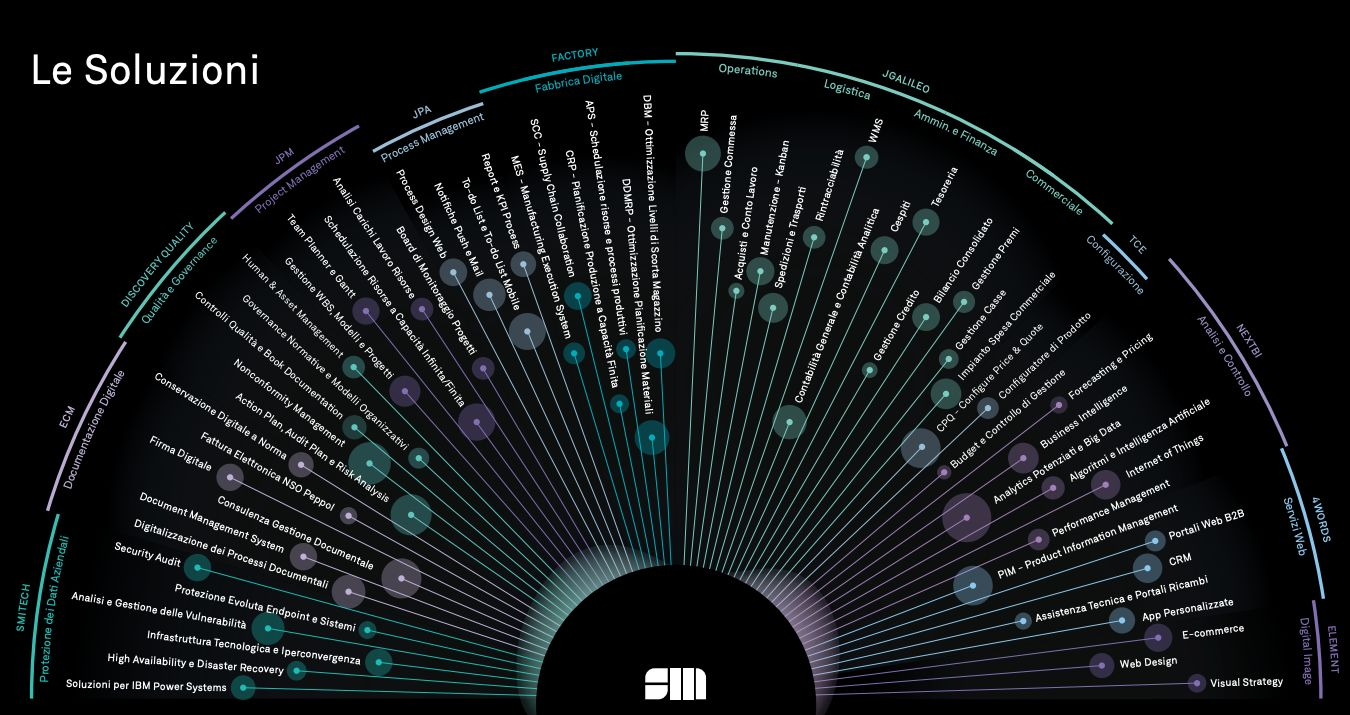
\includegraphics[width=1\columnwidth]{organizzazione-azienda} 
  \caption{Le BU di {\azienda} ed i loro prodotti}
  \label{fig:organizzazione-azienda}
\end{figure}

\noindent Ogni singola BU porta avanti diversi progetti ed ha un responsabile che si occupa di gestire il budget e le risorse umane. \\
\\
Ogni progetto è formato da diverse figure:
\begin{itemize}
  \item Un \gls{PO} che si occupa di gestire il progetto e di interfacciarsi con il cliente;
  \item Uno \gls{Scrum Master} che si occupa di gestire il team di sviluppo e di facilitare il processo di sviluppo;
  \item Gli sviluppatori che si occupano di sviluppare il prodotto;
  \item I tester che si occupano di testare il prodotto;
  \item I consulenti che si occupano di interfacciarsi con il cliente, di capire le sue esigenze e successivamente di installare e configurare il prodotto;
  \item Gli \gls{analisti} che si occupano di analizzare i requisiti del cliente e di redigere la documentazione. Molte volte gli analisti sono anche sviluppatori e tester;
\end{itemize}

\noindent In aggiunta alle componenti precedentemente descritte, ci sono anche altre figure che compongono l'azienda:
\begin{itemize}
  \item \textbf{HR:} si occupa di gestire le risorse umane, di reclutare nuovi dipendenti e di gestire i rapporti con i dipendenti;
  \item \textbf{Marketing:} si occupa di gestire il sito web, i social network e di creare materiale pubblicitario;
  \item \textbf{Amministrazione:} si occupa di gestire la contabilità e le risorse economiche;
  \item \textbf{IT:} si occupa di gestire l'infrastruttura informatica e di fornire supporto ai dipendenti;
  \item \textbf{Commerciali:} si occupano di trovare nuovi clienti e di gestire i rapporti con i clienti esistenti;
  \item \textbf{Direzione:} si occupa di gestire l'azienda e di prendere decisioni strategiche;
  \item \textbf{Centralino:} si occupa di gestire le telefonate e di accogliere i clienti;
  \item \textbf{Presidente:} fondatore dell'azienda, si occupa di prendere decisioni strategiche e di gestire i rapporti con i clienti più importanti;
  \item \textbf{Amministratore delegato:} si occupa di gestire l'azienda e di prendere decisioni strategiche;
\end{itemize}

All'interno dell'azienda c'è una parte di dipendenti che lavora in sede, una parte che lavora in remoto e una parte che lavora presso i clienti. \\
Per riuscire a monitorare il lavoro di tutti i dipendenti, l'azienda utilizza un software di \textit{time tracking} che permette di registrare le ore lavorate. \\
Ogni dipendente ha un proprio \textit{account} che permette di registrare le ore lavorate, di richiedere ferie e permessi. \\
Il software permette di visualizzare le ore lavorate da ogni dipendente e di generare report per ogni progetto e per ogni cliente. \\
Durante l'inserimento delle ore lavorate (Rapporino), il dipendente deve inserire una descrizione delle attività svolte, la commessa, l'eventuale cliente,
la sede in cui ha lavorato, l'ora di inizio e fine lavoro ed eventualmente può collegare il Rapporino ad un ticket. \\
Questa operazione deve essere fatta per ogni giorno lavorativo e ad ogni chiusura del mese vengono bloccate le ore lavorate. \\

\newpage

\section{Il team di sviluppo}
Il team di sviluppo in cui ho lavorato fa parte della BU \textit{JPA} (\textit{Process Management}) e non si
occupa di sviluppare un prodotto specifico, ma ha come obiettivo quello di fornire supporto a tutti i team di sviluppo
dell'azienda. \\
Le principali attività del team sono le seguenti:
\begin{itemize}
  \item \textbf{Supporto:} il team fornisce supporto ai team di sviluppo per la risoluzione di problemi tecnici e analitici;
  \item \textbf{Formazione:} il team fornisce formazione ai team di sviluppo per l'utilizzo di nuovi strumenti e tecnologie;
  \item \textbf{Ricerca e sviluppo:} il team si occupa di sviluppare un \textit{\gls{frameworkg}} interno che permette di creare applicazioni web in modo semplice e veloce;
  \item \textbf{Automazione:} il team si occupa di automatizzare i processi di sviluppo, come ad esempio la compilazione, il rilascio di un prodotto o lo sviluppo di uno nuovo; 
  \item \textbf{Gestione repository:} il team si occupa di gestire i repository di codice sorgente e di fornire supporto per l'utilizzo di strumenti di \textit{\gls{continuous_integrationg}};
  \item \textbf{Installatore:} il team si occupa di sviluppare un installatore per i prodotti dell'azienda che utilizzano il \textit{\gls{frameworkg}} interno;
\end{itemize}

\noindent Il team è composto da 3 persone, uno \gls{Scrum Master} e due sviluppatori. \\
In questo caso sviluppatori sono anche analisti e tester, e molto spesso anche lo \gls{Scrum Master} 
partecipa alle analisi tecniche e funzionali. \\


\section{Strumenti utilizzati}
I principali strumenti per lo sviluppo da me utilizzati sono stati i seguenti:\\
\begin{itemize}
  \item \textbf{Intellij IDEA:} un ambiente di sviluppo integrato (\gls{IDEg}) per il linguaggio di programmazione Java. Fornisce strumenti e funzionalità avanzate per supportare lo sviluppo efficiente del codice, il debug e la testing. Con la sua interfaccia user-friendly e le potenti funzionalità, come l'analisi statica del codice e il refactoring intelligente, IntelliJ IDEA è scelto da molti sviluppatori per creare applicazioni Java professionali;
  \item \textbf{WebStorm:} un IDE per lo sviluppo di applicazioni web, che fornisce un'esperienza di sviluppo ottimale. Grazie alla sua integrazione con strumenti di supporto per lo sviluppo web, come \textit{Node.js}, \textit{Angular}, \textit{React}, WebStorm permette di sviluppare applicazioni web moderne con facilità;
  \item \textbf{Neo4j Desktop:} un programma che permette di installare e gestire database \textit{Neo4j} in modo semplice e veloce. Permette di creare e gestire più database, di monitorare le performance e di eseguire query;
  \item \textbf{Git:} un sistema di controllo versione distribuito, utilizzato per il versionamento del codice sorgente; 
  \item \textbf{Gradle:} un sistema di automazione open source che gestisce le dipendenze e permette di automatizzare il processo di compilazione, testing, pubblicazione e deployment di un software;
  \item \textbf{Docker:} un progetto open source che automatizza il deployment di applicazioni all'interno di contenitori software, fornendo un'astrazione aggiuntiva grazie alla virtualizzazione a livello di sistema operativo di Linux;
  \item \textbf{Bitbucket:} un servizio di hosting per progetti che utilizzano Git come sistema di controllo versione. Fornisce strumenti per la collaborazione e la gestione del codice sorgente;
  \item \textbf{Jenkins:}  un software open source che permette di automatizzare il processo di \textit{build}, testing e deployment di un software;
  \item \textbf{Angular:} un {\gls{frameworkg}} open source per lo sviluppo di applicazioni web, scritto in TypeScript. 
  Fornisce un'architettura \gls{mvvm} e permette di creare applicazioni web dinamiche e scalabili;
  \item \textbf{Jira:} un software di tracciamento dei bug e gestione dei progetti, che permette di pianificare, monitorare e rilasciare software di qualità;
  \item \textbf{Confluence:} un software di collaborazione che permette di creare, organizzare e discutere documenti di progetto;
\end{itemize}

I linguaggi utilizzati sono i seguenti:\\

\begin{itemize}
  \item \textbf{Java:} un linguaggio di programmazione ad alto livello, orientato agli oggetti e a tipizzazione statica, che permette di creare applicazioni web, desktop e mobile;
  \item \textbf{Javascript:} un linguaggio di programmazione ad alto livello, orientato agli oggetti e a tipizzazione dinamica, che permette di creare applicazioni web dinamiche;
  \item \textbf{TypeScript:} un super-set di Javascript che permette di aggiungere tipizzazione statica al linguaggio;
  \item \textbf{Groovy:} un linguaggio di programmazione che permette di scrivere codice che viene eseguito sulla \gls{JVM};
  \item \textbf{Chyper:} un linguaggio di query dichiarativo per grafi, utilizzato per interrogare database \gls{Neo4j};
\end{itemize}

\subsection{Convenzioni}
Per lo sviluppo dei progetti che utilizzano il \textit{frameworkg} interno, sono state definite delle convenzioni da seguire.
Le convenzioni sono salvate all'interno di Confluence, in modo da essere facilmente accessibili a tutti i dipendenti. \\
Sono divise nelle seguenti categorie:
\begin{itemize}
  \item \textbf{Documentazione:} sono delle regole che indica come documentare il codice sorgente, in modo da facilitare la comprensione del codice;
  \item \textbf{Scrittura analisi:} sono delle regole che indicano come scrivere l'analisi dei requisiti e le strutture dell basi di dati, in modo da facilitare la comprensione dell'analisi;
  \item \textbf{Progettazione:} sono delle regole che indicano come progettare i componenti software, in modo da facilitare la manutenzione e l'estensione del codice;
  \item \textbf{Codifica:} sono delle regole che permettono di scrivere codice in modo uniforme, in modo da facilitare la lettura e la comprensione del codice;
  \item \textbf{Versionamento:} sono delle regole che indicano come versionare il codice sorgente, in modo da facilitare la ricerca di una versione specifica del codice;
\end{itemize}

\newpage
\section{Rapporto con l'innovazione}

{\azienda} ha come obiettivo l’innovazione delle aziende clienti per contribuire al loro progresso, 
agevolando la trasformazione digitale ed è specializzata nella progettazione e nella realizzazione di soluzioni integrate, 
a supporto della riorganizzazione di tutti i processi aziendali e professionali.\\
Per raggiungere questo obiettivo, l'azienda indirizza ogni anno dal 15 al 20\% del proprio fatturato all’attività di Ricerca e Sviluppo.\\
Uno dei punti di forza di {\azienda} è la capacità di cogliere le idee e i suggerimenti dei clienti, dei dipendenti, dei collaboratori e trarne ispirazione per sviluppare nuovi prodotti e nuove soluzioni.\\
In questo momento quasi tutti i prodotti attualmente installati presso i clienti hanno una nuova versione in fase di sviluppo,
questo permette all'azienda di essere sempre all'avanguardia e di fornire ai clienti prodotti sempre aggiornati.\\
\\
L'azienda punta molto alla cultura e alla formazione dei propri dipendenti, 
infatti ogni anno vengono organizzati corsi di formazione per permettere ai dipendenti di imparare nuove tecnologie e nuovi strumenti.\\
Questi corsi sono tenuti da dipendenti dell'azienda che hanno già esperienza con le tecnologie e gli strumenti trattati, da consulenti esterni 
o tramite \textit{e-learning}, sulla piattaforma \textit{Udemy Business} messa a disposizione gratuitamente dall'azienda.\\
\\
Inoltre, l'azienda organizza molti eventi dedicati all'innovazione, come ad esempio \textit{Choose Innovation} in collaborazione con \textit{IBM},
dove i vari relatori discutono di innovazione e di come le aziende possono innovare.\\